\section{Auswertung}
\label{sec:Auswertung}



\subsection{Überprüfung der Bragg-Bedingung}
\label{subsec:bragg}
Nach der Bragg-Bedingung ist das gemessene Intensitätsmaximum beim Glanzwinkel von ---- zu erwarten. \\
Dieser liegt bei dem verwendeten KBr-Kristall bei ---- und wird durch die in Tabelle aufgeführten -- Werte der Messung 
verifiziert ???. \\

------- tabelle --------



\subsection{Emissionsspektrum}
\label{subsec:emissionsspektrum}


\subsubsection*{Maximale Energie und minimale Wellenlänge}

Das charakteristische Spektrum der Kupfer-Röntgenröhre ist in Abbildung --- zu sehen.\\
Mit zunehmendem Winkel erkennt man den Grenzwinkel bei  $K_{\alpha}$ und $K_{\beta}$ 
Aus dem Grenzwinkel \begin{equation*}
  \theta_{min} = 
\end{equation*}
lassen sich die maximale Energie und die minimale Wellenlänge \begin{equation*}
  E_{max} = \\\\
  \lambda_{min} =
\end{equation*} 
berechnen.


\subsubsection*{Auflösungsvermögen der Apparatur}

Mit Hilfe der Halbwertsbreite lässt sich auch das Auflösungsvermögen der Apparatur bestimmen. \\
Die Halbwertsbreite berechnet sich aus den Winkeln $\theta_1 = $ und $\theta_2 = $.\\
So ergeben sich die Energien zu $E_1$ und $E_2$, aus deren Differenz $\Delta E = $ keV sich das Auflösungsvermögen
nach ----- zu $A = $ ergibt.


\subsubsection*{Abschirmkonstanten}

Aus den berechneten Energien $E_{K \alpha}$ und $E_{K \beta}$ und dem Literaturwert $E_{K,\;abs} = $ können die Abschirmkonstanten $\sigma_1$, $\sigma_2$ 
und $\sigma_3$ wie folgt bestimmt werden. \\
Aus 
\begin{equation*}
  \sigma_1=Z-\sqrt{\frac{E_{Kabs}}{R_y}}
  \end{equation*}
  
  \begin{equation*}
  \sigma_2=Z-\sqrt{ \frac{m^2}{n^2}(Z-\sigma_1)^2 - \frac{m^2}{R_\infty} E_{K\alpha}}
  \end{equation*}
  
  \begin{equation*}
      \sigma_3=Z-\sqrt{ \frac{l^2}{n^2}(Z-\sigma_1)^2 - \frac{l^2}{R_\infty} E_{K\beta}}
  \end{equation*}
ergeben sie sich zu $\sigma_1 = $, $\sigma_2 = $ 
und $\sigma_3 = $.

\subsection{Absorptionsspektrum}
\label{subsec:absorptionsspektrum}





%\begin{figure}
%  \centering
%  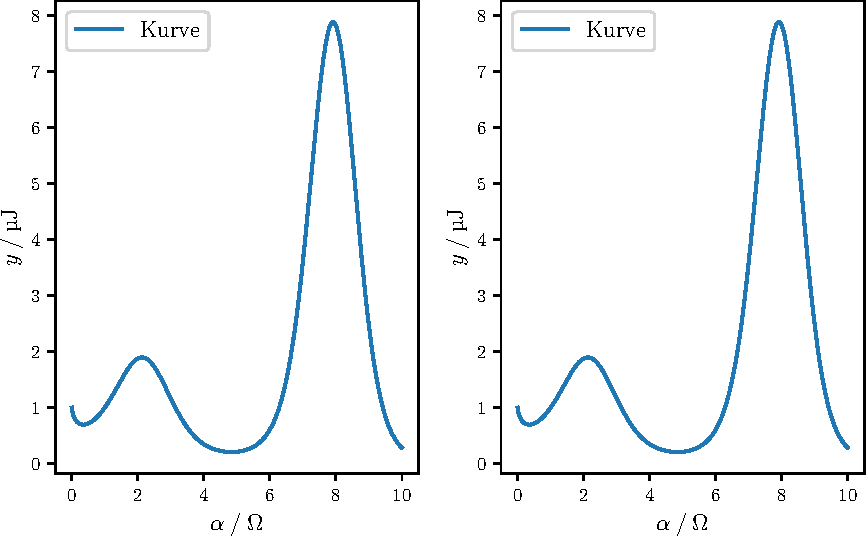
\includegraphics{plot.pdf}
%  \caption{Plot.}
%  \label{fig:plot}
%\end{figure}

%\begin{figure}
%  \centering
%  \includegraphics{build/emissionsspektrum.pdf}
%  \caption{ noch einfügen }
%  \label{fig:plot2}
%\end{figure}



%\begin{figure}
%  \centering
%  \includegraphics{build/moseley.pdf}
%  \caption{Plot.}
%  \label{fig:plot3}
%\end{figure}
%
